\documentclass[a4paper, 12pt]{scrreprt}

\usepackage{amsmath}
\usepackage{amssymb}
\usepackage{amsfonts}
\usepackage{mathrsfs}
\usepackage{graphicx}
\usepackage{float}

\usepackage{varioref}
\usepackage{hyperref}
\usepackage[noabbrev]{cleveref}
\usepackage{booktabs}
\usepackage[utf8]{inputenc}
\usepackage{csquotes}
\usepackage{biblatex}

% Pseudo-codice.
\usepackage{scrhack}
\usepackage{algorithm}
\usepackage{algpseudocode}

\usepackage[T1]{fontenc}

\usepackage[italian]{babel}

\usepackage[headsepline = true, autooneside = false]{scrlayer-scrpage}

\newcommand{\norm}[1]{\left\lVert#1\right\rVert}

\pagestyle{scrheadings}

\lohead{\leftmark}
\cohead{}
\rohead{\rightmark}

\cofoot[]{}
\rofoot[\pagemark]{\pagemark}

\automark[section]{chapter}

\begin{document}

    \title{Algoritmi Distribuiti - prova pratica}
    \date{01/2025}
    \author{Carlo Uguzzoni}

    \maketitle

    \tableofcontents
    \thispagestyle{empty}

    \newpage
    \setcounter{page}{1}

    \chapter{Introduzione}

        Il progetto consiste di un prototipo di file system distribuito (FSD), principalmente basato sull'uso di remote procedure calls (RPC).\\
        L'architettura del sistema si concentra attorno a 3 attori fondamentali:

        \begin{itemize}

            \item Name server: costituisce il fulcro del FSD. Regola le comunicazioni tra clients e file servers, gestisce un database centralizzato contenente i dati dell'intero sistema ed avvia periodicamente task che permettono un funzionamento corretto ed efficiente del sistema

            \item File servers: si occupano dello storage vero e proprio dei files

            \item Clients: utenti del FSD. Gestiscono attivamente i propri files

        \end{itemize}

        Sebbene il name server costituisca un nodo centrale che rappresenta single point of failure (SPOF), il sistema è sviluppato per garantire gestione decentralizzata dei files, scalabilità, replicazione e consistenza.

        \begin{figure}[H]
            \centering
            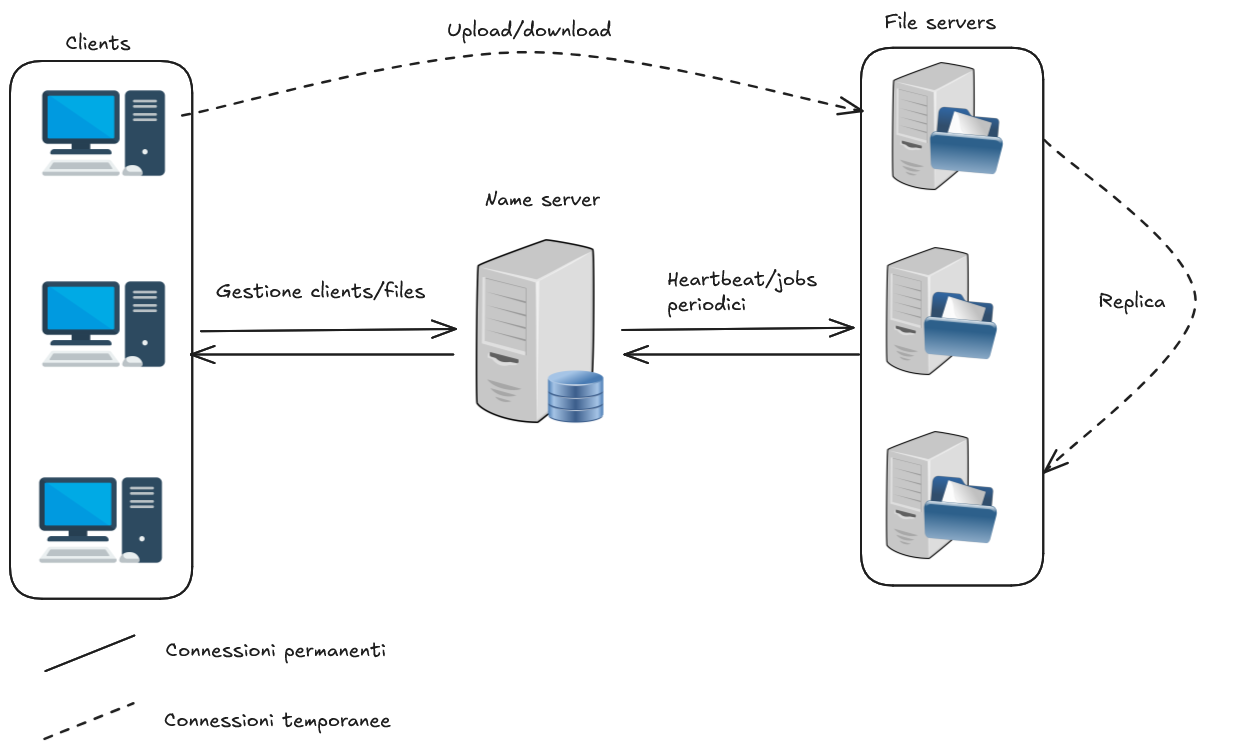
\includegraphics[width = .6 \textwidth]{img/architettura.png}
            \caption{Schema architetturale del sistema}
        \end{figure}

        Il progetto è realizzato in Python, utilizzando la libreria \texttt{RPyC} per l'implementazione delle RPC. Il database del name server viene gestito tramite \texttt{SQLite}, utilizzando l'API di \texttt{sqlite3}.

    \chapter{Architettura}

        \paragraph{Name server}

            Il name server è senz'altro l'entità più importante e complessa del sistema. Si tratta di un oggetto \texttt{rpyc.Service} che fornisce le RPC per rispondere alle richieste dei clients e coordinare le operazioni con i file servers. Queste RPC sono definite con il prefisso \texttt{exposed\_} lato-name server e costituiscono gli unici metodi di quest'entità fruibili alle altre.\\
            Per avviare il name server viene usato un \texttt{ThreadedServer}, che consente di gestire le connessioni simultanee di più clients al servizio. Ogni connessione viene gestita in un thread separato, permettendo il parallelismo e quindi la gestione di richieste concorrenti.\\
            All'avvio del name server vengono anche inizializzati e lanciati tasks periodici, gestiti da un \texttt{BackgroundScheduler} di \texttt{apscheduler}, per le attività di:

            \begin{itemize}

                \item Replica dei files nel DFS: ha lo scopo di mantenere $K$ repliche attive (ovvero in hosting da parte di file servers online) in ogni momento

                \item Check di consistenza dei files: consiste nell'invio ai file servers di una lista dei files loro assegnati e dei relativi checksum, affinché essi possano verificarne la correttezza

                \item Garbage collection: consiste nell'invio ai file servers di una lista dei files loro assegnati, affinché essi possano cancellare dal proprio storage quelli non più necessari

                \item Check di attività delle entità nel DFS: controlla se le entità connesse al name server hanno inviato un heartbeat, che confermasse la propria attività, entro un periodo di tempo fissato. Questo meccanismo ha lo scopo di rilevare e sistemare automaticamente disconnessioni che non seguono un protocollo corretto

            \end{itemize}

            % Se si decide di farlo, una volta sequenzializzati i tasks periodici
            %(in particolare i primi 3), sarà necessario specificare qui o nel
            % seguito perché lo si è fatto ed il loro esatto ordine di esecuzione.

            Il name server è un'entità concepita per essere unica all'interno del sistema. Questa proprietà è garantita tramite l'uso del design pattern "Singleton" e della gestione di un file di lock.\\
            Il progetto supporta un sistema di registrazione e logging sia per i clients che per i file servers. Il file server mette a disposizione tutte le RPC per la gestione delle entità:

            \begin{itemize}

                \item \texttt{exposed\_create\_user} / \texttt{exposed\_create\_file\_server}

                \item \texttt{exposed\_authenticate\_user} / \texttt{exposed\_authenticate\_file\_server}

                \item \texttt{exposed\_delete\_user}

                \item \texttt{exposed\_logout\_user} / \texttt{exposed\_logout\_file\_server}

            \end{itemize}

            All'atto di login delle varie entità presso il name server, viene fornito loro un token di autenticazione, firmato con una chiave privata nota solo al name server stesso. Il payload del token contiene nome e ruolo dell'entità che esegue il login. Il suo scopo è quello di implementare un sistema di ruoli, permessi ed autenticazione a cui sottoporre chi chiama le RPC critiche per la sicurezza. Ad esempio, senza questo meccanismo un client regolare potrebbe richiamare le RPC di un amministratore, o peggio quelle che regolano i meccanismi di replica dei files. La chiave pubblica con la quale decriptare il payload è inoltrata ai file servers che eseguono il login, affinché anche questi possano sottoporre a controllo le chiamate in ingresso. Nello specifico, i token sono JSON Web Tokens (JWT), firmati con chiavi RSA da 2048 bit.\\
            Un elemento fondamentale del name server è il database centrale, che contiene tutte le informazioni necessarie al corretto funzionamento del sistema. In esso viene conservato lo stato di clients, file servers, files e repliche.\\
            Il file server attinge alle informazioni nel database per convalidare login/logout delle entità, portare a termine la loro creazione/cancellazione, eseguire i tasks periodici, indirizzare la comunicazione tra clients e file servers, e molto altro. Il database centrale consiste in un file SQLite, che viene gestito tramite l'API di \texttt{sqlite3}.

            \begin{figure}[H]
                \centering
                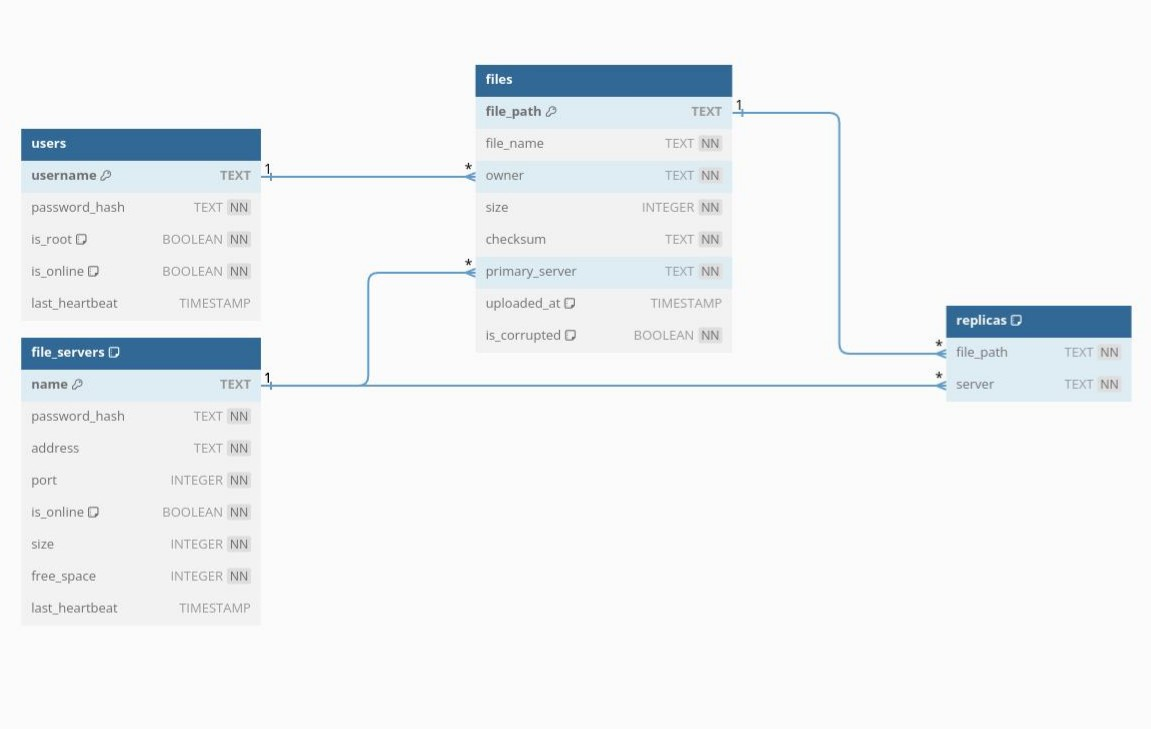
\includegraphics[width = 1. \textwidth]{img/ERD.jpg}
                \caption{ERD del database centrale}
            \end{figure}

            Il name server interagisce con i clients tramite diverse RPCs:

            \begin{itemize}

                \item \texttt{exposed\_get\_user\_files}: restituisce la lista dei files di un utente

                \item \texttt{exposed\_get\_file\_server\_upload}: restituisce le coordinate (\texttt{ip}, \texttt{port}) di un file server per l'upload di un file, scegliendolo con il metodo "K-least loaded". Il file server su cui viene caricato il file verrà marcato come "primary" per tale file

                \item \texttt{exposed\_get\_file\_server\_download}: restituisce le coordinate (\texttt{ip}, \texttt{port}) di un file server per il download di un file, dando priorità al file server marcato come "primary" per tale file

                \item \texttt{exposed\_delete\_file}: cancella un file dal sistema. La cancellazione avviene solo nel database, il task di garbage collection provvederà all'eliminazione effettiva del file dal FSD

                \item \texttt{exposed\_get\_file\_server\_update}: restituisce le coordinate (\texttt{ip}, \texttt{port}) di un file server per l'aggiornamento di un file. L'update di fatto consiste in una sequenza di cancellazione ed upload, per garantire immediata disponibilità del servizio più replicazione e consistenza alla prima chiamata dei tasks periodici

                \item \texttt{exposed\_list\_all\_files}: esclusiva del client amministratore, restituisce la lista di tutti i files e le relative repliche presenti nel sistema

                \item \texttt{exposed\_list\_all\_clients}: esclusiva del client amministratore, restituisce la lista di tutti i clients nel sistema ed il loro stato

                \item \texttt{exposed\_list\_all\_file\_servers}: esclusiva del client amministratore, restituisce la lista di tutti i file servers nel sistema ed il loro stato

            \end{itemize}

            Task periodici e altre funzioni di handling vengono approfonditi e descritti nel seguito.

        \paragraph{File server}

            I file servers realizzano lo storage vero e proprio nel FSD. Essi ereditano a loro volta da \texttt{rpyc.Service} e vengono lanciati da un \texttt{ThreadedServer}.\\
            Per i file servers è prevista un'interfaccia a riga di comando che consente la registrazione di un nuovo file server od il login di un file server esistente.\\
            Il sistema, pur essendo scalabile di default, è concepito per realizzare un FSD di piccole dimensioni. Per questo motivo non è possibile la cancellazione di un file server esistente, come avviene per i clients. La sua implementazione sarebbe in realtà un task relativamente semplice, che implicherebbe la rimozione del file server da ruolo di "primary" per tutti i files attualmente assegnati e la successiva ri-assegnazione degli stessi ad uno nuovo. Infine, si dovrebbero cancellare tutte le repliche assegnate al file server ed il suo record dalle tabelle del database.\\
            La connessione con il name server avviene all'avvio. Devono essere forniti come parametri \texttt{host} e \texttt{port} del name server allo script di lancio.\\
            Nonappena avviene con successo il login, il file server avvia il loop principale e diventa disponibile per le richieste. Lo spegnimento deve avvenire tramite un segnale di terminazione; viene gestita l'uscita in modo polite con \texttt{SIGINT}.\\
            I file servers ineragiscono con i clients tramite le RPCs:

            \begin{itemize}

                \item \texttt{exposed\_store\_file}

                \item \texttt{exposed\_send\_file}

            \end{itemize}

            che ricevono/inviano rispettivamente un file. Come già indicato, i clients vengono appositamente indirizzati dal name server, prima di accedere a queste RPC.\\
            Il salvataggio ed il reperimento dei files avvengono sullo stesso host del file server in una directory predefinita. La directory di base assegnata a ciascun client coincide con il suo \texttt{username} nel database centrale.\\
            L'interazione tra file servers e name server è invece più complessa. Abbiamo:

            \begin{itemize}

                \item \texttt{exposed\_send\_file\_replicas}: chiamata dal job di replicazione periodica, si occupa di inviare repliche di un file ad una lista di altri file servers

                \item \texttt{exposed\_garbage\_collection}: chiamata dal job di garbage cleaning periodico, elimina files non più presenti sul database del name server e tutte le directory vuote

                \item \texttt{exposed\_consistency\_check}: chiamata dal job di consistency check periodico, controlla la consistenza dei file presenti sul database del name server. Se riconosce un'incongruenza, chiama una speciale RPC del name server per risolverla

            \end{itemize}

            In ultimo, i file servers, quando attivi, inviano periodicamente un heartbeat al name server per confermare la loro attività. Lo heartbeat è schedulato come job periodico in un \texttt{BackgroundScheduler}.

        \paragraph{Regular client}

            I clients regolari rappresentano gli utenti standard del FSD. Le loro facoltà sono principalmente quelle di eseguire upload/download/listing di files sul FSD tramite le RPC messe a disposizione dalle entità server. La connessione con il name server avviene all'avvio.\\
            L'interfaccia da riga di comando consente ai regular clients di eseguire liberamente login/logout e di autenticarsi con diversi profili. I files sono salvati sullo stesso host dal quale i clients si autenticano, in una directory predefinita. La directory di base di ciascun utente coincide con il suo \texttt{username} nel database centrale.\\
            All'upload di un file è richiesto al client di specificare il percorso assoluto del file da caricare e la directory di destinazione all'interno del FSD. In questo modo è possibile caricare nel FSD un file da qualsiasi directory locale.\\
            Nel download si richiede il solo percorso del file nel FSD. Il file viene scaricato nella base directory locale del client autenticato, assieme a tutta la struttura di directories da cui discende nel FSD.

        \paragraph{Root clients}

            Il client root dispone di tutte le funzionalità garantite ai clients di regolari (cioè quelle di base), infatti entrambi ereditano dalla classe astratta \texttt{BaseClient}. Inoltre, può richiamare RPC esclusive per visualizzare lo stato di tutte le entità ed i files nel FSD. Queste funzionalità assolvono principalmente alla funzione di amministrazione e manutenzione del FSD.\\
            Per ora al client root non sono garantiti accesso, cancellazione ed upload di files dei clients regolari, in quanto queste azioni sono critiche dal punto di vista della privacy degli utenti. Si potrebbero implementare in futuro, per esempio a patto che il loro uso venga rigorosamente registrato da un apposito sistema di logging.\\
            Il client root è pensato per essere unico nel FSD, che come abbiamo detto è concepito per avere modeste dimensioni. Come per il name server, si è adottato il design pattern Singleton, con annesso meccanismo basato su file di lock. È dunque possibile effettuare una sola volta la registrazione per questo ruolo ed il login è statico.\\
            Come i file servers, tutti i clients (anche quelli regolari) inviano periodicamente un heartbeat al name server per confermare la loro attività.

    \chapter{Interazioni}

        \paragraph{Upload e download}

            Queste sono senz'altro le due interazioni più comuni nell'uso del FSD che coinvolgono direttamente ed attivamente i clients e le entità server.\\
            Nel primo caso, il client chiama il metodo RPC \texttt{exposed\_get\_file\_server\_upload} del name server. Quest'ultimo interroga il database centrale e restituisce le coordinate di un file  server online in grado di ricevere il file. Come abbiamo detto, tale file server viene marcato come "primary". Ciò significa che sarà il primo a ricevere il file, il punto di riferimento per le repliche e la prima scelta in caso di download. A questo punto, il client si connette direttamente al file server indicato, richiamando la RPC \texttt{exposed\_store\_file}, che provvede a trasferire il file generando, se necessario, tutta la struttura di directories.\\
            La procedura di download segue una dinamica del tutto analoga. Il client si rivolge al name server con la RPC \texttt{exposed\_get\_file\_server\_download}, che fornisce le coordinate del primary server del file specificato, o quelle di un altro file server se questo non è online. Il client si connette al file server, richiamando la RPC \texttt{exposed\_send\_file} per ottenere il file.

            \begin{figure}[H]
                \centering
                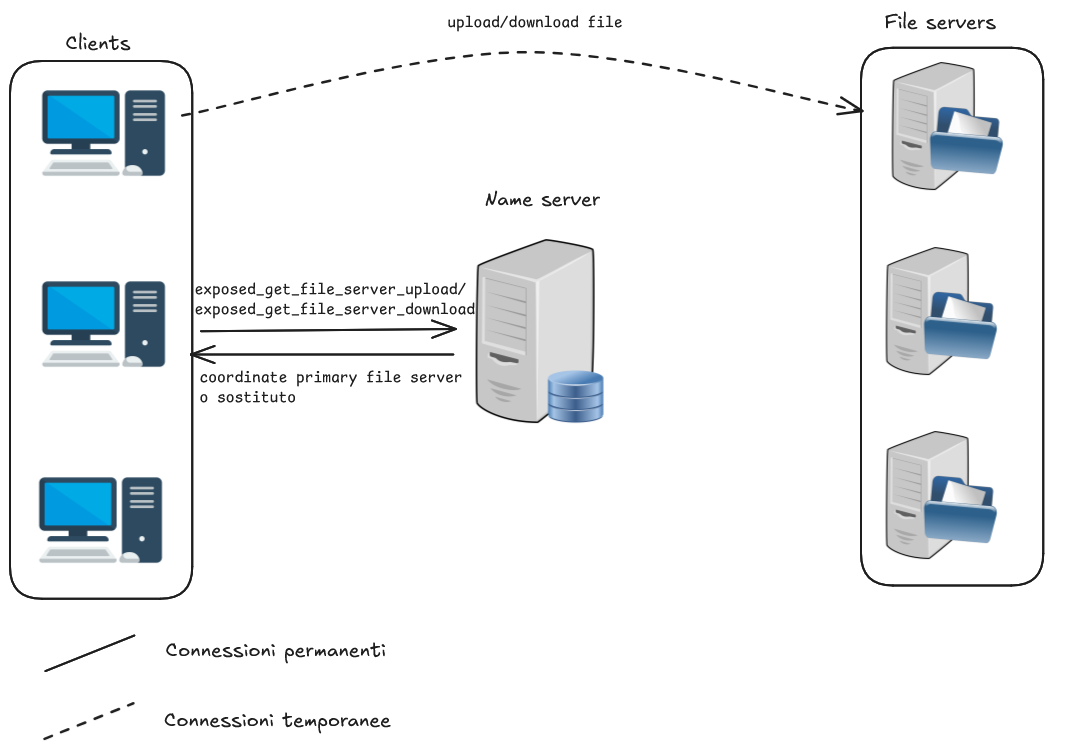
\includegraphics[width = .6 \textwidth]{img/upload_download.png}
                \caption{Interazioni clients/servers per upload/download}
            \end{figure}

        \paragraph{Tasks periodici}

            % Opzionale introduzione all'ordine dei tasks periodici e al master job.

            \subparagraph{Replicazione}

                La replicazione riguarda tutti quei files che hanno meno di $K$ repliche attive, ovvero presenti su meno di $K$ file servers online. Questi vengono selezionati dal name server, assieme alle coordinate (ovvero la coppia \texttt{host}, \texttt{port}) del relativo primary server. Il name server chiama quindi la RPC \texttt{exposed\_send\_file\_replicas}, allegando le coordinate di tutti i file servers online che non ospitano già una replica del file, per raggiungere un massimo di $K$ in totale.\\
                A questo punto, il primary file server, iterativamente, invia il file ai nuovi file servers tramite la RPC \texttt{exposed\_store\_file}.\\
                Una volta restituita al chiamante la prima RPC, vengono create le entry nella tabella \texttt{replicas} del database centrale. Repliche non andate a buon fine vengono successivamente eliminate dai tasks di consistency check e garbage cleaning.

                \begin{figure}[H]
                    \centering
                    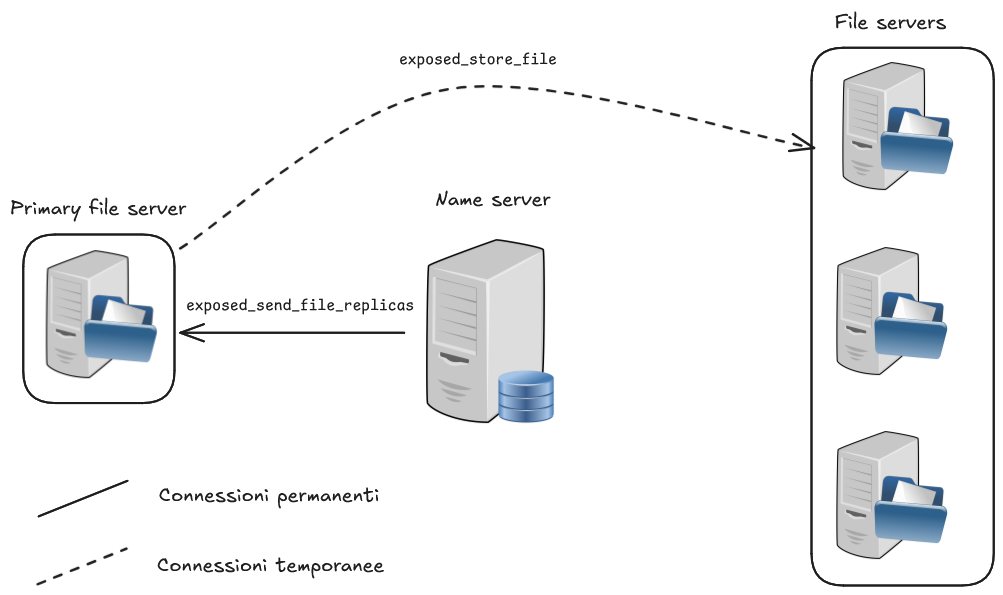
\includegraphics[width = .6 \textwidth]{img/replica.png}
                    \caption{Interazioni name server/file servers per replicazione}
                \end{figure}

            \subparagraph{Check di consistenza}

                Il name server invia a tutti i file servers i nomi dei files in essi salvati ed i relativi checksums, così che questi possano controllarne l'integrità. Questo processo avviene tramite la chiamata della RPC \texttt{exposed\_consistency\_check}.\\
                Nel caso il checksum calcolato sul file nello storage del file server non corrisponda a quello fornito dal name server, oppure il file non venga trovato, il file server chiama una apposita RPC del name server per gestire l'inconsistenza operando sul database centrale. Questa RPC è \texttt{exposed\_handle\_inconsistency}.\\
                Nel caso di inconsistenza, il name server cancella la replica sul file server chiamate, così che questa venga rimossa dal successivo garbage cleaning. Dopodiché, se si trattava di un file server primario ne assegna uno nuovo al file, dando priorità a quelli online che ne ospitano una copia. In caso contrario, la procedura termina.\\
                Se non viene trovato alcun file server contenente una replica per il file, esso viene marcato come \texttt{corrupted}. I files corrotti non possono più essere reperiti dai clients, ma solo cancellati. I clients possono conoscere lo stato di ogni file di loro proprietà tramite la lista dei propri files sul FSD.

                \begin{figure}[H]
                    \centering
                    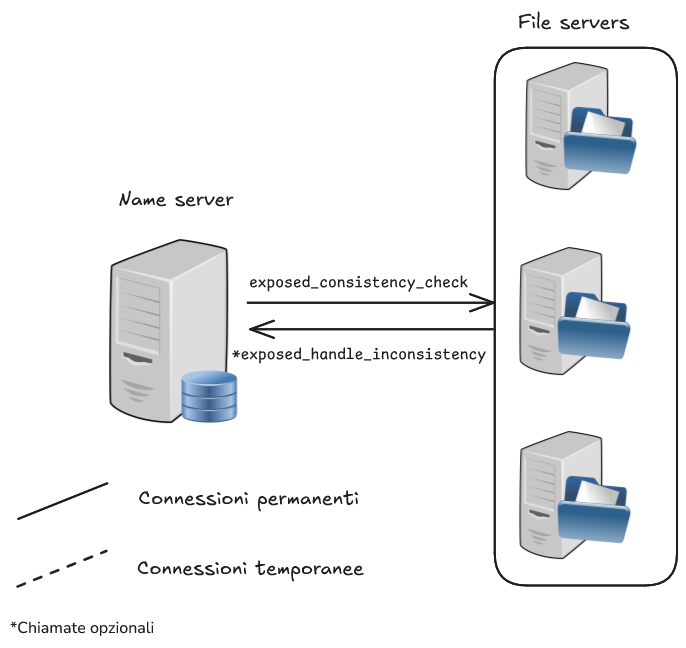
\includegraphics[width = .4 \textwidth]{img/consistency.png}
                    \caption{Interazioni name server/file servers per check di consistenza}
                \end{figure}

            \subparagraph{Garbage cleaning}

                Il name server invia a tutti i file servers i nomi dei files in essi salvati. Questi nomi consistono in realtà del campo \texttt{file\_path} della tabella \texttt{files}, ovvero del path assoluto dei files nel FSD.\\
                I file servers rimuovono tutti i files nel proprio storage che non compaiono nella lista ricevuta dal name server, più le directories rimaste vuote a seguito della rimozione.

            \subparagraph{Eventual consistency}

                Il concetto di eventual consistency è stato formalmente definito da Werner Vogels come segue: \textit{"Se non vengono eseguite nuove operazioni di aggiornamento, dopo un tempo sufficientemente lungo tutte le repliche del sistema convergeranno allo stesso stato"}.\\
                Nel FSD realizzato, il name server, attraverso l'esecuzione dei tasks periodici descritti sopra, garantisce questa proprietà.

                \begin{itemize}

                    \item La replica fornisce ridondanza e disponibilità

                    \item Il consistency check realizza sincronizzazione tra i files, prendendo come riferimento privilegiato il file server primario

                    \item Il garbage cleaning rimuove files incongruenti per evitare incoerenza tra le repliche

                \end{itemize}

                In questo modo, anche in presenza di fallimenti temporanei o partizioni di rete, tutte le repliche alla fine rifletteranno uno stato coerente con la visione del name server.

    \chapter{Conclusioni}

        In questo progetto è stato realizzato un FSD con un’architettura fortemente centralizzata, in cui il name server gestisce la mappatura dei file, coordina le interazioni tra clients e file servers, e svolge varie operazioni per garantire consistenza.\\
        Tra i propri punti di forza il sistema offre:

        \begin{itemize}

            \item Gestione centralizzata: riduce la complessità delle classi che non sono il name server e la logica delle interazioni tra loro

            \item Un sistema di tasks periodici, i quali:

            \begin{itemize}

                \item Delegano per design quanto più lavoro possibile ai file servers, riducendo il carico sul name server e cercando di dare scalabilità al sistema

                \item Garantiscono eventual consistency, oltre che tolleranza ai guasti e disponibilità

            \end{itemize}

        \end{itemize}

        Tuttavia, sono presenti anche diverse limitazioni:

        \begin{itemize}

            \item SPOF: il funzionamento del name server è essenziale per quello dell'intero sistema, dunque una possibile rottura potrebbe rendere il tutto inutilizzabile

            \item Scalabilità limitata: un'architettura fortemente centralizzata come quella proposta, con l'aggiunta di un alto numero di nodi potrebbe risentire pesantemente del carico di lavoro sul name server. Sebbene si sia cercato di scaricare il name server da ogni lavoro superfluo e comunque il sistema sia concepito per avere dimensioni limitate, questa problematica rimane una possibilità concreta

        \end{itemize}

        Una soluzione possibile a queste problematiche, perlopiù architetturali, potrebbe essere quella rifattorizzare l'intero progetto introducendo una nuova architettura completamente distribuita, ad esempio basata su Distributed Hash Tables (DHT). Anche il modello di consistenza potrebbe essere migliorato, aderendo a standard più potenti, pur incrementando significativamente la complessità del progetto.\\
        In ultimo, se invece si pensasse che l'architettura attuale sia sufficiente per servire allo scopo, una modifica applicabile per migliorare le performances potrebbe essere la parallelizzazione del lancio dei tasks periodici, che nella versione base è sequenziale. Realizzare questa feature per l'hardware sul quale è stato realizzato il progetto non avrebbe avuto molto senso, anche perché i file servers attivi erano tipicamente al massimo 3 (sempre per la natura modesta del sistema).

\end{document}